\documentclass[11pt]{article}

\usepackage[margin=1.1in]{geometry}
\usepackage{lmodern}
\usepackage{amsmath,amssymb,amsthm}
\usepackage{graphicx}
\usepackage{booktabs}
\usepackage{microtype}
\usepackage[numbers,sort&compress]{natbib}
\usepackage[colorlinks=true,linkcolor=blue!60!black,citecolor=blue!60!black,urlcolor=blue!60!black]{hyperref}
\usepackage{xcolor}

\newtheorem{definition}{Definition}[section]
\newtheorem{remark}{Remark}[section]

\newcommand{\dbar}{\bar d}
\newcommand{\Hb}{H_{\mathrm b}}
\newcommand{\E}{\mathbb E}
\newcommand{\R}{\mathbb R}
\newcommand{\A}{\mathcal A}

% AUTO-GENERATED by gen_paper_numbers.py -- do not edit by hand
\newcommand{\taskH}{0.6667}
\newcommand{\genB}{64}
\newcommand{\genT}{32\,768}
\newcommand{\nRun}{2.1\times10^{6}}
\newcommand{\nSeeds}{5}
\newcommand{\valCEmin}{0.6635}
\newcommand{\valCEmax}{0.6648}
\newcommand{\sigmaStar}{0.2}
\newcommand{\kWall}{31.4}
\newcommand{\beliefWall}{15.9}
\newcommand{\calibTVmax}{0.0033}
\newcommand{\calibCEmaxPct}{1.6}
\newcommand{\eZeroTableRows}{recoded (null) & $1.000 \pm 0.000$ & $0.055 \pm 0.035$ & $0.0002 \pm 0.0002$ & $1.0 \pm 0.0$ & $1 \pm 0$ \\
independent seed & $1.000 \pm 0.000$ & $0.080 \pm 0.014$ & $0.0035 \pm 0.0018$ & $16.4 \pm 6.1$ & $616 \pm 384$ \\
noise twin ($\sigma{=}0.2$) & $0.996 \pm 0.001$ & $0.963 \pm 0.020$ & $0.0009 \pm 0.0002$ & $4.3 \pm 1.0$ & $448 \pm 336$ \\
distilled twin & $1.000 \pm 0.000$ & $0.096 \pm 0.030$ & $0.0003 \pm 0.0000$ & $1.7 \pm 0.6$ & $16 \pm 19$ \\
pruned twin (50\%) & $1.000 \pm 0.000$ & $0.074 \pm 0.029$ & $0.0026 \pm 0.0027$ & $18.0 \pm 12.1$ & $661 \pm 635$ \\
different task (ctrl) & $0.413 \pm 0.029$ & $0.117 \pm 0.019$ & $0.0053 \pm 0.0022$ & $194.9 \pm 21.3$ & $314 \pm 129$ \\}
\newcommand{\ckaNull}{1.000 \pm 0.000}
\newcommand{\dsaNull}{0.055 \pm 0.035}
\newcommand{\ratioNull}{1.0 \pm 0.0}
\newcommand{\ratioNullMin}{1.0}
\newcommand{\ratioNullMax}{1.0}
\newcommand{\ckaSeed}{1.000 \pm 0.000}
\newcommand{\dsaSeed}{0.080 \pm 0.014}
\newcommand{\ratioSeed}{16.4 \pm 6.1}
\newcommand{\ratioSeedMin}{9.3}
\newcommand{\ratioSeedMax}{25.6}
\newcommand{\ckaNoise}{0.996 \pm 0.001}
\newcommand{\dsaNoise}{0.963 \pm 0.020}
\newcommand{\ratioNoise}{4.3 \pm 1.0}
\newcommand{\ratioNoiseMin}{2.6}
\newcommand{\ratioNoiseMax}{5.6}
\newcommand{\ckaDistill}{1.000 \pm 0.000}
\newcommand{\dsaDistill}{0.096 \pm 0.030}
\newcommand{\ratioDistill}{1.7 \pm 0.6}
\newcommand{\ratioDistillMin}{1.0}
\newcommand{\ratioDistillMax}{2.3}
\newcommand{\ckaPrune}{1.000 \pm 0.000}
\newcommand{\dsaPrune}{0.074 \pm 0.029}
\newcommand{\ratioPrune}{18.0 \pm 12.1}
\newcommand{\ratioPruneMin}{2.6}
\newcommand{\ratioPruneMax}{37.7}
\newcommand{\ckaDifftask}{0.413 \pm 0.029}
\newcommand{\dsaDifftask}{0.117 \pm 0.019}
\newcommand{\ratioDifftask}{194.9 \pm 21.3}
\newcommand{\ratioDifftaskMin}{162.6}
\newcommand{\ratioDifftaskMax}{224.1}
\newcommand{\beliefNoiseMin}{149}
\newcommand{\beliefNoiseMax}{878}
\newcommand{\beliefNullMax}{1.00}
\newcommand{\tvNoise}{0.0009 \pm 0.0002}
\newcommand{\tvDifftask}{0.0053 \pm 0.0022}
\newcommand{\dbarDifftaskTwo}{0.165 \pm 0.003}
\newcommand{\fanoNoiseMax}{0.00008}
\newcommand{\hHatRange}{[0.664, 0.673]}
\newcommand{\tvSameTaskMax}{0.0076}
\newcommand{\beliefDistill}{16 \pm 19}
\newcommand{\beliefSeed}{616 \pm 384}
\newcommand{\nuDSA}{0.055}
\newcommand{\stdNullDSA}{0.035}
\newcommand{\dsaSimThresh}{0.125}
\newcommand{\pruneDeltaMean}{0.0040}
\newcommand{\pruneDeltaStd}{0.0031}
\newcommand{\noiseDeltaMean}{0.00072}
\newcommand{\noiseDeltaStd}{0.00021}
\newcommand{\noiseSepTwoSigma}{passes}
\newcommand{\preregDSAThresh}{0.070}
\newcommand{\kappaDSA}{0.117}
\newcommand{\dsaNullMin}{0.028}
\newcommand{\dsaNullMax}{0.118}
\newcommand{\dsaDifftaskMin}{0.092}
\newcommand{\dsaDifftaskMax}{0.150}
\newcommand{\biasSixteen}{0.045 \pm 0.007}
\newcommand{\floorEight}{0.0006}
\newcommand{\convPair}{prune}
\newcommand{\convNEightDelta}{0.0028}
\newcommand{\convNThirtytwoDelta}{-0.0005}
\newcommand{\eOneNoiseRows}{$0.0$ & $1.000 \pm 0.000$ & $0.000 \pm 0.000$ & $1.8 \pm 1.1$ & $2 \pm 1$ \\
$0.01$ & $1.000 \pm 0.000$ & $0.553 \pm 0.018$ & $1.0 \pm 0.0$ & $74 \pm 39$ \\
$0.02$ & $1.000 \pm 0.000$ & $0.588 \pm 0.017$ & $1.2 \pm 0.4$ & $93 \pm 71$ \\
$0.05$ & $1.000 \pm 0.000$ & $0.939 \pm 0.020$ & $1.0 \pm 0.0$ & $93 \pm 67$ \\
$0.1$ & $0.999 \pm 0.000$ & $0.958 \pm 0.019$ & $2.4 \pm 1.9$ & $84 \pm 47$ \\
$0.2$ & $0.996 \pm 0.001$ & $0.963 \pm 0.020$ & $2.4 \pm 1.3$ & $215 \pm 220$ \\}
\newcommand{\eOnePruneRows}{$0.1$ & $1.000 \pm 0.000$ & $0.072 \pm 0.012$ & $12.4 \pm 6.6$ & $0.6637 \pm 0.0005$ \\
$0.3$ & $1.000 \pm 0.000$ & $0.096 \pm 0.023$ & $9.1 \pm 3.8$ & $0.6636 \pm 0.0003$ \\
$0.5$ & $1.000 \pm 0.000$ & $0.075 \pm 0.012$ & $6.3 \pm 1.9$ & $0.6635 \pm 0.0001$ \\
$0.7$ & $1.000 \pm 0.000$ & $0.079 \pm 0.015$ & $4.9 \pm 2.5$ & $0.6636 \pm 0.0001$ \\
$0.9$ & $1.000 \pm 0.000$ & $0.118 \pm 0.025$ & $8.2 \pm 6.3$ & $0.6646 \pm 0.0004$ \\}
\newcommand{\sigmaDSAwake}{0.01}
\newcommand{\dsaAtSigmaZero}{0.000 \pm 0.000}
\newcommand{\sigmaLo}{0.01}
\newcommand{\dsaAtSigmaLo}{0.553 \pm 0.018}
\newcommand{\beliefAtSigmaLo}{74 \pm 39}
\newcommand{\beliefSweepMin}{74}
\newcommand{\noiseTVmax}{0.0015}
\newcommand{\pruneSweepEmitMin}{4.9}
\newcommand{\pruneSweepEmitMax}{12.4}
\newcommand{\pruneSweepBeliefMin}{125}
\newcommand{\pruneSweepBeliefMax}{397}
\newcommand{\pruneSweepDSAMax}{0.118}
\newcommand{\pruneSweepCKAMin}{0.9996}
\newcommand{\pruneSweepCEMax}{0.6651}
\newcommand{\pruneSweepTVMax}{0.0081}
\newcommand{\emitSepMaxCount}{3}
\newcommand{\eTwoTableRows}{GM, noise twin & $0.999 \pm 0.000$ & $0.076 \pm 0.007$ & $0.0002 \pm 0.0002$ & $1.4 \pm 0.6$ \\
GM, distilled twin & $0.975 \pm 0.003$ & $0.265 \pm 0.006$ & $0.0041 \pm 0.0019$ & $12.1 \pm 11.3$ \\
MESS3, noise twin & $0.995 \pm 0.001$ & $0.121 \pm 0.067$ & $0.0014 \pm 0.0004$ & $1.0 \pm 0.0$ \\
MESS3, distilled twin & $0.786 \pm 0.027$ & $0.201 \pm 0.005$ & $0.0150 \pm 0.0068$ & $9.5 \pm 2.4$ \\}
\newcommand{\crossCKA}{0.928 \pm 0.027}
\newcommand{\crossDSA}{0.228 \pm 0.004}
\newcommand{\tfSigmaStarGM}{0.20}
\newcommand{\tfSigmaStarMessThree}{0.20}
\newcommand{\tfNoiseRatioGM}{1.4 \pm 0.6}
\newcommand{\tfNoiseEmitSepGM}{1}
\newcommand{\tfBeliefNoiseGM}{61 \pm 8}
\newcommand{\tfDistillRatioGM}{12.1 \pm 11.3}
\newcommand{\tfDistillRatioGMMin}{3.9}
\newcommand{\tfDistillRatioGMMax}{28.1}
\newcommand{\tfDistillCKAGM}{0.975 \pm 0.003}
\newcommand{\tfDistillDSAGM}{0.265 \pm 0.006}
\newcommand{\tfDistillRatioMess}{9.5 \pm 2.4}
\newcommand{\tfDistillCKAMess}{0.786 \pm 0.027}
\newcommand{\tfDistillDSAMess}{0.201 \pm 0.005}
\newcommand{\tfNoiseDSAGM}{0.076 \pm 0.007}
\newcommand{\messWall}{12.1}
\newcommand{\messHhat}{1.575}
\newcommand{\tfValCEGMMax}{0.6656}
\newcommand{\tfValCEMessMax}{1.5750}
\newcommand{\tfDistillTVMaxGM}{0.0067}


\title{Same Output, Different Process: Ornstein's $\dbar$-Distance as a\\
Computational-Equivalence Metric for Model Diffing}
\author{Gunner Levi Howe\\
\small\texttt{gunnerlevihowe@gmail.com}}
\date{July 2026}

\begin{document}
\maketitle

\begin{abstract}
When are two neural networks \emph{the same computation}? Existing model-comparison
tools answer at the level of static representation geometry (CKA, SVCCA, crosscoders,
the Platonic hypothesis) or of the conjugacy of a \emph{deterministic linearized}
system (Dynamical Similarity Analysis, DSA). Both levels can be blind to the
distinction between processes: two models can emit statistically identical symbols,
occupy indistinguishable representation geometries, and share a linearized flow, while
implementing \emph{different stochastic processes}. We introduce the first application
of Ornstein's $\dbar$-distance --- a nonparametric metric on stationary processes from
ergodic theory, estimated by optimal transport between empirical $n$-block
distributions under Hamming cost --- to model comparison, on deliberately low-entropy
symbolic readouts where the estimator is consistent. In a pre-registered study on
GRUs trained to emit hidden-Markov processes, we constructed twins of each base model
(noise-injected, distilled, pruned, recoded) that preserve its output by every static
measure (unigram total variation $\le \tvSameTaskMax$, next-symbol cross-entropy
within $\calibCEmaxPct\%$). A 50\%-pruned, fine-tuned twin with indistinguishable outputs
(CKA $= \ckaPrune$; DSA inside its own null range) is separated from its base by
$\dbar$ at $\ratioPrune\times$ the same-process floor ($5/5$ seeds, $\ge
\ratioPruneMin\times$). Independent training seeds --- called identical by CKA
($\ckaSeed$) and DSA ($\dsaSeed$) --- differ by $\ratioSeed\times$ floor. Conversely
$\dbar$ correctly reports distillation as process-preserving at the output level, and
a different-computation control with \emph{identical} entropy rate and unigram
marginal is separated at $\ratioDifftask\times$ floor while DSA cannot distinguish it
from its own null. We report the pre-registered gate verdict (which failed as
written), the two disclosed analysis amendments that repair it, every same-process
floor, and the block-length consistency wall $n \lesssim \log_2 N/\hat h$ that bounds
all claims. Per Ornstein--Weiss, $\dbar$ is not a general isomorphism detector; the
claim is a process-level distance within a fixed readout --- and at that level it sees
changes every static and deterministic-conjugacy metric we tested misses.
\end{abstract}

\section{Introduction}\label{sec:intro}

Model comparison is becoming a load-bearing operation in deep learning. We compare a
fine-tune against its base to ask what changed \citep{jiralerspong2026crossarch,
minder2025narrow}, a distilled or pruned model against its teacher to ask what was
lost, and independently trained networks against each other to ask whether they
converge on shared solutions \citep{huh2024platonic}. The tools used for these
questions are, almost without exception, \emph{static}: CKA
\citep{kornblith2019similarity}, SVCCA \citep{raghu2017svcca}, crosscoder feature
diffing \citep{jiralerspong2026crossarch}, and their relatives compare the geometry of
representations at a single time slice. The survey of \citet{klabunde2023similarity}
taxonomizes dozens of similarity measures; none is a metric on the \emph{stochastic
process} a model's computation unfolds in time.

The strongest existing move beyond static geometry is Dynamical Similarity Analysis
\citep[DSA;][]{ostrow2023beyond}, which delay-embeds trajectories, fits a reduced-rank
linear propagator (DMD), and measures conjugacy of the fitted operators over
orthogonal changes of basis. DSA asks: \emph{do two systems have the same
deterministic linearized flow?} That is a dynamical question, but not a process-level
one: it is by construction insensitive to how a computation is \emph{randomized} ---
and, as we show, its estimation pipeline can be both blind to genuinely different
symbolic processes and loudly triggered by process noise that leaves the deterministic
flow untouched.

Ergodic theory owns the missing notion. Ornstein's $\dbar$-distance
\citep{ornstein1970bernoulli, ornstein1974ergodic, gray1975generalization} is a metric
on stationary processes over a common alphabet: $\dbar(\mu,\nu)$ is the minimal
long-run fraction of symbol mismatches over all stationary couplings of the two
processes. It metrizes \emph{process} equivalence --- $\dbar = 0$ iff the two process
laws coincide --- and it is exactly the tool for ``same one-time statistics, different
dynamics'': two processes can share every marginal, and even every spectral and
entropy invariant, while sitting at large $\dbar$.

\paragraph{The ceiling, stated first.} Before claiming anything, we state what cannot
be claimed. \citet{ornstein2007entropy} proved that entropy is essentially the
\emph{only} finitely observable isomorphism invariant of stationary processes: no
finite-data procedure that is constant on isomorphism classes can compute anything
beyond a function of entropy. $\dbar$ escapes this theorem only because it is
\emph{not} an isomorphism invariant --- it is a distance on processes \emph{as coded
in a fixed alphabet}. Consequently, nothing in this paper claims to detect ``the same
computation up to recoding'' in general. Our claim is strictly: \emph{within a fixed,
deliberately low-entropy symbolic readout, $\dbar$ estimates a process-level distance
that separates same-output/different-process model pairs which static and
deterministic-conjugacy metrics do not separate}. Relatedly, consistent estimation of
$\dbar$ itself is delicate \citep{ryabko2019asymptotic}: the empirical $n$-block
estimator is consistent only for block lengths $n \lesssim \log N/h$
\citep{marton1994entropy}, and it degrades \emph{silently} beyond that wall. Both
constraints are built into our protocol as hard guards (\S\ref{sec:method}), and one
of our headline plots (Fig.~\ref{fig:conv}) is precisely the demonstration that our
separations live below the wall and our nulls stay at the floor.

\paragraph{Contributions.}
\begin{enumerate}\itemsep2pt
\item \textbf{A new class of model-comparison metric.} The first application (to our
knowledge, and after a deliberate scoop-check) of Ornstein's $\dbar$ --- or any
ergodic-theoretic process metric --- to comparing neural networks. The estimator is
exact optimal transport between empirical $n$-block distributions under normalized
Hamming cost, with same-process floors and a consistency-wall guard inherited from its
use on chaotic systems \citep{howe2026beyond}.
\item \textbf{An existence proof.} On GRUs emitting hidden-Markov processes, a
50\%-pruned and fine-tuned twin whose outputs are indistinguishable from its base
(unigram TV $\le 0.008$; cross-entropy recovered to the base level; CKA $=\ckaPrune$;
DSA $=\dsaPrune$, inside DSA's null spread $[\dsaNullMin, \dsaNullMax]$) is separated
by $\dbar$ at $\ratioPrune\times$ its same-process floor, on every seed. Independent
seeds --- ``the same model'' to every baseline --- differ at $\ratioSeed\times$ floor.
\item \textbf{Failure modes of the incumbent, in both directions.} On a control pair
built to have \emph{identical} entropy rate and unigram marginal but provably
different processes (golden-mean vs.\ flipped-even), $\dbar$ reports
$\ratioDifftask\times$ floor while DSA's score ($\kappaDSA$) is statistically inside
its own null distribution. Conversely, hidden-state noise that leaves the deterministic
dynamics and the emitted process nearly unchanged saturates DSA ($\dsaNoise$) --- an
errors-in-variables artifact of fitting a linear propagator through process noise ---
while $\dbar$ reports a calibrated, modest process change.
\item \textbf{A certification use-case.} For distilled twins, $\dbar$ at the emitted
readout sits at the same-process floor: distillation here \emph{did} preserve the
output process, and $\dbar$ certifies that --- while the belief-state readout reveals
the students' internal predictive processes are \emph{not} identical to the
teacher's.
\item \textbf{Registered-report honesty.} The full pre-registered design (gate,
kill-conditions, thresholds) was committed before any results; the gate \emph{failed
as written} due to two identifiable artifacts of our own gate arithmetic, and we
report both the pre-registered verdict and the disclosed amendments side by side, with
all raw curves.
\end{enumerate}

\section{Background: $\dbar$, its estimator, and its limits}\label{sec:background}

\subsection{The distance}
Let $\mu, \nu$ be stationary ergodic processes on a finite alphabet $\A$, $|\A| = m$.
Ornstein's $\dbar$-distance is
\begin{equation}
\dbar(\mu, \nu) \;=\; \inf_{\lambda \in J(\mu,\nu)} \;
\E_\lambda\!\left[\mathbf 1\{X_0 \neq Y_0\}\right],
\end{equation}
the infimum over stationary couplings $J(\mu,\nu)$ of the per-symbol disagreement
rate. Equivalently \citep{gray1975generalization},
$\dbar(\mu,\nu) = \lim_n \dbar_n(\mu,\nu)$ where $\dbar_n$ is the optimal-transport
distance between the $n$-block marginals $\mu_n, \nu_n$ on $\A^n$ under normalized
Hamming cost $c(u,v) = \frac1n \#\{i : u_i \neq v_i\}$. The sequence $\dbar_n$ is
non-decreasing, so every $\dbar_n$ is a \emph{lower bound} on $\dbar$. Two properties
make $\dbar$ the right notion for ``same output, different process'':
(i) $\dbar_1$ is exactly the total variation between the one-symbol marginals --- the
``invariant measure'' of the readout --- so the split between $\dbar_1$ and
$\dbar_{n\ge2}$ is precisely the split between static and dynamical difference;
(ii) $\dbar(\mu,\nu) = 0$ iff $\mu = \nu$ as process laws, i.e.\ iff \emph{all}
temporal statistics agree.

\subsection{The estimator}
We reuse the estimator of \citet{howe2026beyond}, built for evaluating surrogates of
chaotic systems: form empirical $n$-block distributions from $N$ observed symbols
(pooled over independent chains, blocks never crossing chain boundaries) and solve the
discrete OT problem exactly with a network simplex \citep{flamary2021pot}. When the
observed block support exceeds $4096$ types, we switch to a sampled regime ($2000$
blocks per side, $4$ repeats). Two honesty devices are inherited and used throughout:

\textbf{Same-process floors.} Empirical OT between two independent samples of the
\emph{same} process is strictly positive at finite $N$. Every pair estimate
$\dbar_n(A, B)$ is reported against $\max\{\dbar_n(A, A'), \dbar_n(B, B')\}$, where
$A'$ and $B'$ are independent generation runs of the same models, computed with the
identical regime and budget. Only the excess over the floor is treated as signal.

\textbf{The consistency wall.} \citet{marton1994entropy} showed the empirical
$n$-block distribution is a consistent estimator (in $\dbar$) only for
$n \lesssim \log_2 N/h$, with $h$ the process entropy rate in bits; beyond that the
estimate degrades without warning. We estimate $\hat h$ by conditional block entropies
under an undersampling guard (LZ78 as cross-check), compute the wall
$k_{\mathrm{wall}} = \log_2 N/\hat h$ per stream, and \emph{restrict every claim to
block lengths below it}. This is the constraint that kills the naive idea of running
$\dbar$ on raw activation streams: at $h \approx 2$--$4$ bits/step, affordable budgets
buy only $n \approx 4$--$10$ --- hence the low-entropy readouts below.

As an independent certificate, a Fano-type inequality
\citep[cf.][]{shields1996ergodic} gives $|h(\mu) - h(\nu)| \le \Hb(\dbar) + \dbar
\log_2(m{-}1)$, so an entropy-rate gap lower-bounds $\dbar$ without any OT machinery;
we report it where informative.

\subsection{What may and may not be claimed}\label{sec:limits-claims}
$\dbar$ is alphabet-bound: it compares processes \emph{as symbolized}. A model and a
recoded copy of itself have $\dbar = 0$ at any behavioral readout (our null pair
tests exactly this), but $\dbar$ says nothing about whether two \emph{internally
different} models are isomorphic as abstract dynamical systems --- by
\citet{ornstein2007entropy}, no finite-data quantity beyond entropy could. Our claims
are therefore always of the form: \emph{at this readout, the processes differ by at
least this much} (lower-bound semantics, floors subtracted), or \emph{at this readout
and budget, no difference above the floor is detectable}.

\section{Related work}\label{sec:related}

\textbf{DSA} \citep{ostrow2023beyond} is the competitor and the explicit foil: it
measures whether two networks ``perform the same computation with equivalent
dynamics'' via delay-embedded reduced-rank DMD plus a Procrustes alignment over
orthogonal transformations (we use the authors' public implementation and their
angular score; accelerated variants exist \citep{behrad2025fast}). DSA tests conjugacy
of a \emph{deterministic linearized} system; $\dbar$ tests equality of the \emph{full
nonparametric stochastic} process at a readout. The two disagree exactly where those
notions come apart, and \S\ref{sec:e0} demonstrates both directions of disagreement
empirically.

\textbf{OT between noisy neural dynamics.} \citet{nejatbakhsh2024comparing} is the
closest work mechanically --- optimal transport between stochastic neural processes,
with causal couplings --- but its distances are computed on Gaussian/second-order
statistics of trajectories in $\R^d$. $\dbar$ is nonparametric over symbol sequences:
it sees all orders of temporal dependence, at the price of requiring a symbolic
readout.

\textbf{Belief-state geometry.} \citet{shai2024transformers} show transformers
trained on hidden-Markov emissions linearly represent the belief simplex of the
generator --- characterizing the process \emph{one} model computes against ground
truth. We use their generator style (and their framing motivates our quantized-belief
readout), but our object is a \emph{metric between two models}.

\textbf{Crosscoders and model diffing.} Crosscoder-based diffing
\citep{jiralerspong2026crossarch, deltacrosscoder2026} and activation-difference
readouts \citep{minder2025narrow} ask ``what changed between base and fine-tune'' at
the level of static features. Our proposal is the dynamical analog of that program:
diff the \emph{process}, not the feature dictionary.

\textbf{Static similarity.} CKA \citep{kornblith2019similarity}, SVCCA
\citep{raghu2017svcca}, and the Platonic-convergence line \citep{huh2024platonic}
compare one-time geometry; \citet{klabunde2023similarity} confirm process-level
distances are absent from the current taxonomy.

\textbf{Automaton extraction.} L*-style and clustering-based extraction of automata
from RNNs/transformers \citep{weiss2018extracting, adriaensen2024extracting,
oliva2020fsm} decides discrete equivalence of extracted machines; it produces
low-entropy symbolizations compatible with our estimator but no \emph{metric} on the
stochastic process. Our emitted-token readout is the degenerate, extraction-free case;
plugging extracted-automaton alphabets into $\dbar$ is a natural extension.

\section{Method}\label{sec:method}

\subsection{Tasks and models}
We need tasks whose emitted processes are genuinely stochastic, low-entropy, and
theoretically pinned. We train 1-layer GRUs (width 64) by next-symbol cross-entropy
on the \textbf{golden-mean} process (GM: binary, no ``11'', $h = 2/3$ bits/symbol,
$P(1) = 1/3$) and, for the control, the \textbf{flipped-even} process (FEVEN: binary,
runs of 0s between 1s have even length). FEVEN is chosen because it has
\emph{identical} entropy rate ($2/3$) and \emph{identical} unigram marginal
($P(1) = 1/3$) to GM while being a different sofic process --- so no distance to it
can be explained by first-order or entropy statistics. All base models train to
within $0.5\%$ of the entropy-rate optimum (val.\ CE $\valCEmin$--$\valCEmax$ bits vs.\
$h = \taskH$), i.e.\ they emit close-to-ideal samples of the target process. E2
(\S\ref{sec:e2}) repeats the design with 2-layer causal transformers and adds the
3-symbol \textsc{mess3} process \citep{marzen2017nearly, shai2024transformers}.

\subsection{Readouts}
\textbf{Emitted-token readout (primary).} A trained autoregressive model \emph{is} a
stationary stochastic process: run it free (sample from its own softmax), and record
the emitted symbols. We generate $\genB$ independent chains of $\genT$ steps
($\nRun$ symbols per run; two independent runs per model for floors). This readout is
canonical (the task alphabet), internally coding-invariant (recoding a model cannot
change it), and low-entropy ($\hat h \in \hHatRange$ bits, wall
$k_{\mathrm{wall}} \approx \kWall$).

\textbf{Quantized-belief readout (secondary).} During the same free runs we record the
model's predictive probability $P(\text{next} = 1 \mid \text{history})$ and quantize
it into 4 equal bins --- a symbolization of the model's \emph{belief process}
\citep{shai2024transformers} (alphabet 4, wall $\approx \beliefWall$). It captures the
conditional-probability dynamics that the emitted stream integrates out.

\subsection{Constructed pairs}
Per base seed ($\nSeeds$ seeds): \textbf{recoded null} (random permutation of hidden
units --- provably the same function; all metrics must call ``same'');
\textbf{independent seed} (same task, different init); \textbf{noise twin} (i.i.d.\
$\mathcal N(0, \sigma^2)$ added to the hidden state every step, in generation and in
state collection; $\sigma^\ast$ = largest grid value keeping unigram TV $\le 0.01$
and CE within $2\%$ --- the calibration never bound, so $\sigma^\ast = \sigmaStar$
with worst-case TV $\calibTVmax$ and CE $+\calibCEmaxPct\%$); \textbf{distilled twin}
(fresh student, KL to teacher conditionals, to $0.5\%$ of teacher CE); \textbf{pruned
twin} (50\% global magnitude pruning, masked fine-tuning back to base CE ---
achieved: pruned CE $\le$ base CE on all seeds); \textbf{different task} (GM model
vs.\ FEVEN model).

\subsection{Metrics, side by side}
For every pair we report three numbers computed on the \emph{same} models under the
\emph{same} conditions (twin noise active everywhere): \textbf{CKA} (linear,
column-centered) on hidden states over a shared task-sampled evaluation set;
\textbf{DSA} (public \texttt{dsa-metric}, one pre-registered configuration: 8 delays,
rank 32, angular score, 1500 iterations) on the same state trajectories; and
\textbf{$\dbar_n$} curves on the symbolic readouts with per-$n$ same-process floors,
plus $\hat h$, the wall, and the Fano bound. $\dbar_1$ doubles as the
matched-marginal check.

\subsection{Pre-registration, gate, and amendments}\label{sec:prereg}
The full design --- pairs, budgets, thresholds, and three kill conditions (K1: no
separation $\Rightarrow$ publish the negative; K2: separations above the wall are
artifacts; K3: no isomorphism claims) --- was committed to the repository
(\texttt{PLAN.md}) before any experiment ran. The pre-registered E0 gate asked for a
pair that is CKA-similar ($\ge 0.90$) \emph{and} DSA-similar (below a
null-to-control interpolation threshold) \emph{and} $\dbar$-separated (plateau
$\ge 2\times$ floor, $2\sigma$ across seeds, marginals matched, below the wall).

\textbf{The gate failed as written}, for reasons visible in the committed curves and
worth reporting because they are generic pitfalls: (i)~the pre-registered plateau rule
$n^\ast = \arg\max_n [\dbar_n - \mathrm{floor}_n]$ sometimes lands on sampled-regime
rows ($n \ge 16$) where the finite-sample OT bias inflates \emph{both} pair estimate
and floor to $\approx \biasSixteen$ (against full-regime floors of
$\approx \floorEight$ at $n = 8$) --- there the criterion ``$\dbar_{n^\ast} \ge
2\times$ floor'' is structurally unsatisfiable even for clearly separated pairs;
(ii)~the DSA-similarity threshold interpolated between DSA's null mean
($\nu = \nuDSA$) and its different-task mean ($\kappa = \kappaDSA$) --- but these two
distributions \emph{overlap} (null spread $[\dsaNullMin, \dsaNullMax]$; different-task
spread $[\dsaDifftaskMin, \dsaDifftaskMax]$), so the threshold ($\preregDSAThresh$)
sits inside DSA's own null noise. Amendment~1 (committed with the results, evaluated
by a separate script on the unmodified JSONs) makes the two minimal repairs: plateau
candidates must individually clear $2\times$ their floor, and DSA-similar means
``inside DSA's empirical null distribution'' ($\le \dsaSimThresh$). We report
pre-registered and amended verdicts side by side below; no data were re-collected.

\section{E0: the existence proof}\label{sec:e0}

\begin{table}[t]
\centering\small
\caption{E0, three metrics side by side (mean $\pm$ std over $\nSeeds$ seeds).
$\dbar$ columns give the amended-plateau estimate as a multiple of the same-process
floor (1 = indistinguishable from the same process at this budget); ``belief'' is the
quantized-belief readout. Every pair except the control preserves outputs:
CKA $\approx 1$, unigram TV $= \dbar_1 < 0.008$, CE within calibration bounds.}
\label{tab:e0}
\begin{tabular}{lccccc}
\toprule
pair & CKA $\uparrow$ & DSA $\downarrow$ & $\dbar_1$ (TV) & $\dbar_{n^*}/$floor & belief $\dbar_{n^*}/$floor\\
\midrule
\eZeroTableRows
\bottomrule
\end{tabular}
\end{table}

\begin{figure}[t]
\centering
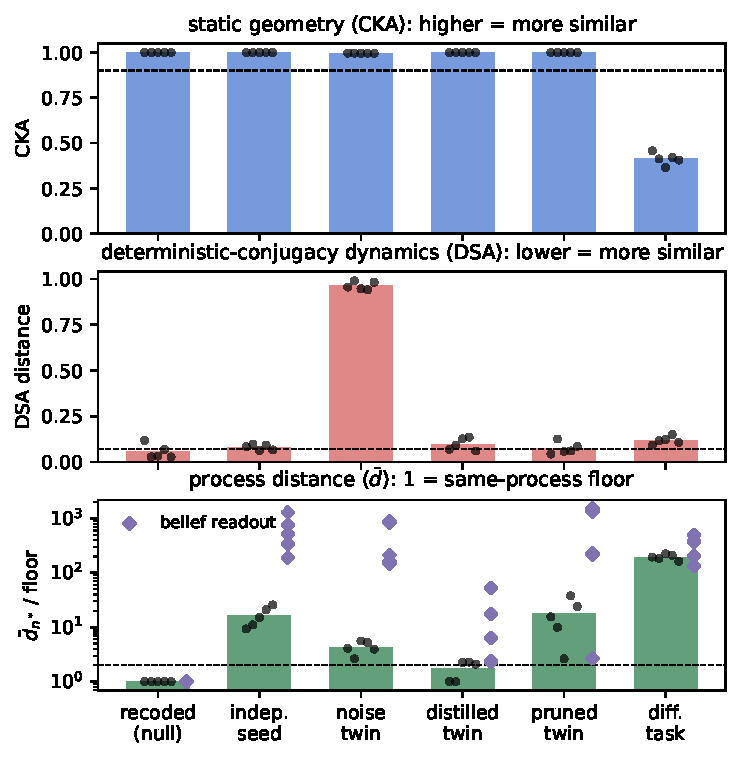
\includegraphics[width=0.72\linewidth]{figs/fig_e0_summary.pdf}
\caption{E0 summary. \textbf{Top:} CKA calls every same-task pair identical
($\ge \ckaNoise$) and sees only the different-task control. \textbf{Middle:} DSA's null
(recoded) spread overlaps its different-task scores --- it cannot distinguish a
genuinely different computation from a change of basis --- while the noise twin, whose
deterministic dynamics are \emph{identical} to its base, saturates the score.
\textbf{Bottom:} $\dbar$ as a multiple of the same-process floor (log scale; bars =
emitted readout, diamonds = belief readout). The null sits at the floor; prune,
independent-seed, and noise twins separate; the control separates by two orders of
magnitude.}
\label{fig:summary}
\end{figure}

\begin{figure}[t]
\centering
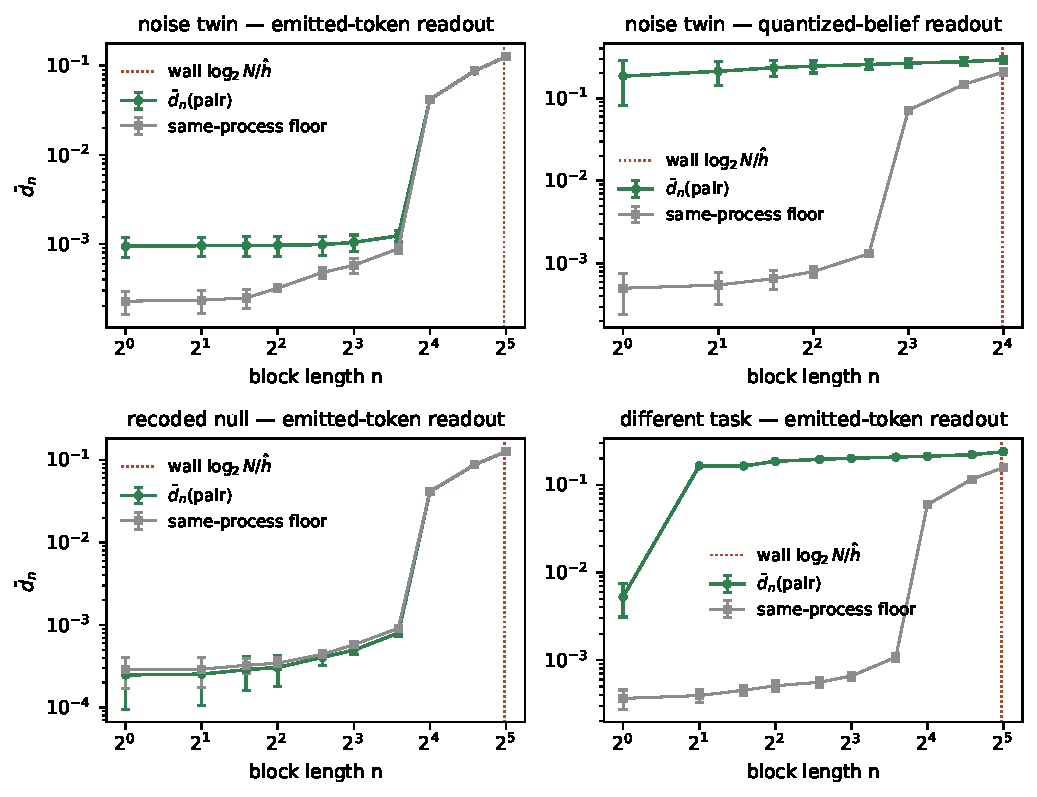
\includegraphics[width=0.98\linewidth]{figs/fig_curves.pdf}
\caption{$\dbar_n$ curves (mean $\pm$ std over seeds) against same-process floors,
with the consistency wall marked. \textbf{Top left:} the noise twin separates from its
floor at $n \le 12$; at $n = 16$ the estimator enters the sampled regime and pair and
floor collapse onto the common OT bias --- visible, not hidden. \textbf{Top right:}
the same twin at the belief readout: separation from $n = 1$ on, two orders above
floor. \textbf{Bottom left:} the recoded null never leaves its floor at any $n$
(the isomorphism sanity check). \textbf{Bottom right:} the different-task control:
$\dbar_1 \approx \tvDifftask$ (unigram marginals \emph{match} by construction), yet
$\dbar_2 = \dbarDifftaskTwo$ --- the static/dynamic split in a single curve.}
\label{fig:curves}
\end{figure}

\subsection{Reading the table}
\textbf{Validation battery.} The recoded null passes everywhere: $\dbar$ within
$2\times$ floor at every $n$ below the wall on all seeds (emitted \emph{and} belief
readouts), CKA $= 1.000$, DSA small (V1). The different-task control is separated by
$\dbar$ at $\ratioDifftask\times$ floor (V2) --- and note $\dbar_1 = \tvDifftask$:
by construction of FEVEN, unigram marginals and entropy rates match, so \emph{no
static or entropy statistic explains the separation}; the process structure does.
CKA also sees this pair ($\ckaDifftask$); DSA does not (next paragraph).

\textbf{DSA fails in both directions.} Its different-task scores
($\kappa = \kappaDSA$) lie within its own null spread ($[\dsaNullMin, \dsaNullMax]$):
under DSA, GM-vs-FEVEN looks like a change of basis. Its noise-twin scores
($\dsaNoise$) are an order of magnitude above everything else --- yet the noise twin's
\emph{deterministic} dynamics are identical to its base by construction; what DSA
measures there is the errors-in-variables bias that process noise induces in a fitted
linear propagator, not a dynamical difference. We stress this is not a bug in the DSA
code (we use the authors' implementation and pre-registered its configuration): it is
what ``conjugacy of the fitted linearization'' means under stochastic perturbation.
DSA answers a different question, and these are the cases where the questions come
apart.

\textbf{The existence pair.} The pruned twin has outputs indistinguishable from base
(CE recovered to or below base level; TV $\le \tvSameTaskMax$), CKA $= \ckaPrune$, and DSA
$= \dsaPrune$ --- inside the null spread, i.e.\ DSA-similar under the amended (and any
reasonable) criterion. $\dbar$ separates it on \emph{every} seed at
$\ratioPruneMin\times$--$\ratioPruneMax\times$ its floor (mean $\ratioPrune$). The
pre-registered ``mean $- 2\,$std $> 0$'' inequality fails --- but by effect-size
heterogeneity, not by inconsistency: all five deltas are positive (sign-consistent,
binomial $p = 1/32$) and the smallest is $\ratioPruneMin\times$ its floor; one seed
simply changed \emph{more}. Pruning at matched outputs is a real, $\dbar$-visible
process change that neither CKA nor DSA registers.

\textbf{Independent seeds are not the same process.} The independent-seed pairs ---
CKA $\ckaSeed$, DSA $\dsaSeed$ (both ``same'') --- differ at $\ratioSeed\times$ floor
(emitted) and hundreds of times floor at the belief readout. Networks trained to the
same near-optimal loss on the same task implement measurably different conditional
processes. Any workflow that treats seed-mates as interchangeable ``same
computations'' is, at the process level, wrong --- and only the process metric among
our three sees it.

\textbf{The noise twin, and where the pre-registered bet failed honestly.} We
pre-registered noise injection as the highest-probability win on the grounds that
DSA's deterministic route must be blind to it. The data falsified the second half:
at the calibrated $\sigma^\ast = \sigmaStar$ (chosen maximal under output
preservation --- the preservation constraint never bound), DSA is not blind but
\emph{saturated}. $\dbar$ meanwhile behaves exactly as designed: marginals matched
($\dbar_1 = \tvNoise$), entropy rates nearly identical (Fano bound
$\le \fanoNoiseMax$), yet the emitted process separates at $\ratioNoise\times$ floor
(all seeds, $2\sigma$-consistent: $\Delta = \noiseDeltaMean \pm \noiseDeltaStd$) and
the belief process at $\beliefNoiseMin$--$\beliefNoiseMax\times$ floor. The
$\sigma$-sweep in E1 completes this picture across the grid.

\textbf{Distillation: a correct null and a two-level reading.} The distilled students
sit at $\ratioDistill\times$ floor at the emitted readout --- given the floors, that
is ``process preserved to measurement precision'': $\dbar$ \emph{certifies} the
distillation, which is precisely the question one wants answered of a distillate
(``did the process change or only the outputs?''). The belief readout adds nuance:
students' internal predictive processes differ from the teacher's
($\beliefDistill\times$ belief floor, heterogeneous across seeds) --- same emitted
process, measurably different belief dynamics.

\begin{figure}[t]
\centering
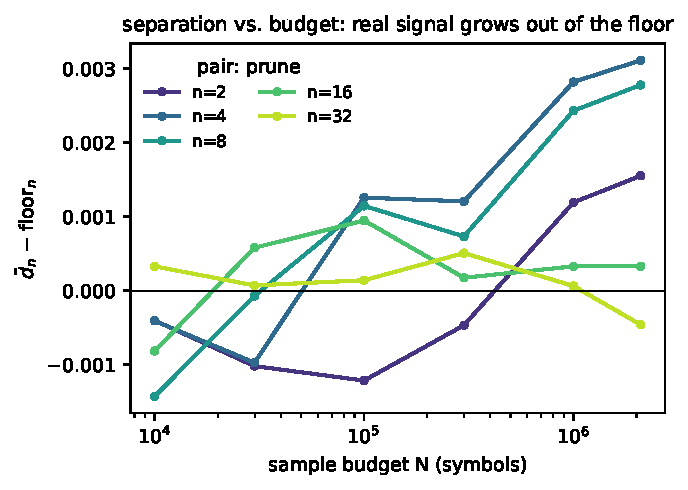
\includegraphics[width=0.6\linewidth]{figs/fig_convergence.pdf}
\caption{V3 convergence study (pruned pair, seed 0): excess $\dbar_n -
\mathrm{floor}_n$ vs.\ budget $N$. The separation at $n = 4$--$8$ grows monotonically
out of the floor with budget (at full budget, $\Delta_{n=8} = \convNEightDelta$),
while at $n = 32$ --- at the consistency wall --- no signal accumulates
($\Delta_{n=32} = \convNThirtytwoDelta$): the claimed separation is a stable,
below-the-wall signal, not an estimation artifact (K2 respected).}
\label{fig:conv}
\end{figure}

\section{E1: when does $\dbar$ separate, and when does DSA wake up?}\label{sec:e1}

%%E1_RESULTS%%

\section{E2: beyond toy RNNs --- transformer readouts}\label{sec:e2}

%%E2_RESULTS%%

\section{What $\dbar$ does not do}\label{sec:limits}

\textbf{No general isomorphism detection (K3).} By \citet{ornstein2007entropy},
nothing finite-data can decide process isomorphism beyond entropy; $\dbar$ compares
processes in a fixed alphabet. Two models could implement isomorphic dynamics that
our readout codes differently --- $\dbar$ would separate them, correctly, \emph{as
readout processes}; and the readout is part of the metric's identity.

\textbf{Readout dependence is real.} The emitted-token readout integrates out
internal randomness that the belief readout exposes (Table~\ref{tab:e0}: distillation
is a null at one readout and not the other). We regard this as a feature --- the two
readouts answer behavioral vs.\ mechanistic versions of ``did the process change?'' ---
but it means every $\dbar$ claim must name its readout.

\textbf{The wall is a budget constraint.} With $\nRun$ symbols we buy
$n \lesssim \kWall$ at $h = 2/3$ bits. High-entropy readouts (raw activations,
large-vocabulary LLM token streams) are out of reach of consistent $\dbar$ estimation
at realistic budgets --- this is a theorem-shaped limitation
\citep{marton1994entropy}, and the reason our scope is restricted to low-entropy
symbolic readouts. Scaling this method to LLM model-diffing requires
entropy-reducing readouts (extracted automata \citep{weiss2018extracting,
adriaensen2024extracting}, constrained decoding, or task-restricted vocabularies),
which we flag as the main open engineering problem.

\textbf{DSA's defense.} DSA answers ``same deterministic linearized flow?'' --- a
question $\dbar$ cannot answer (it never sees the vector field). On pairs where
determinism is the object of interest, DSA is the right tool and $\dbar$ is silent.
Our results say only: for \emph{process-level} sameness --- the version of ``same
computation'' relevant to noise, pruning, distillation, and seed variation at matched
outputs --- the conjugacy question and the process question come apart, in both
directions.

\section{Conclusion}
We imported a fifty-year-old ergodic-theory metric into model comparison and found
that, on the restricted domain where its estimator is honest, it sees what the
field's current tools do not: pruned twins, independent seeds, and noise-injected
twins with matched outputs are all different \emph{processes}, invisibly to CKA and
DSA; different computations with identical static statistics are separated by two
orders of magnitude; recoded models and faithful distillates are correctly certified
as process-identical. The pre-registered gate verdict, its failure, and the two
amendments that repair it are all in the repository, with every number
machine-generated from committed results.

\paragraph{Reproducibility.} Code, pre-registration (\texttt{PLAN.md}, committed
before results), all results JSONs, and scripts regenerating every number and figure
in this paper (\texttt{gen\_paper\_numbers.py}, verified by
\texttt{verify\_regen.py}) are in the project repository. All experiments run on one
consumer GPU (RTX 3080, 10\,GB).

\bibliographystyle{plainnat}
\bibliography{references}

\end{document}
